\documentclass[english, 12pt, a4paper, sci, utf8, a-1b, online]{aaltothesis}
% testi
\usepackage{graphicx}

\usepackage{amsfonts, amssymb, amsbsy, amsmath}
\usepackage[english, finnish]{babel}
\usepackage{natbib}

\usepackage{csvsimple}

\usepackage{caption}
\usepackage{subcaption}

\newpage

\bibliographystyle{plainnat}
\setcitestyle{authoryear,open={(},close={)}}

\degreeprogram{Engineering Physics and Mathematics}

\major{Mathematics and Systems Sciences}

\code{SCI3029}

\univdegree{BSc}


\thesisauthor{Leevi Rönty}

\thesistitle{Bayesian model validation metrics in retail datasets}

\place{Espoo}
\date{14.10.2020}

\supervisor{Prof.\ Fabricio Oliveira}

\advisor{DSc\ (Tech.) Mikko Ervasti}
\advisor{DSc\ (Tech.) Paavo Niskala} % TODO: checkaa voiko tähän lisätä kahta näin

\uselogo{aaltoBlue}{''}


\keywords{Bayesian models\spc model validation\spc
	information criterion\spc Facebook Prophet}

\thesisabstract{
Tiivistelmässä on lyhyt selvitys kirjoituksen tärkeimmästä sisällöstä: mitä ja
miten on tutkittu, sekä mitä tuloksia on saatu. Tämän opinnäytteen 
tiivistelmäteksti kirjoitetaan opinnäytteen luettavan osan
lomakkeen lisäksi myös pdf-tiedoston metadataan. Kirjoita tähän metadataan
kirjoitettavaa teksti. Metadatatekstissa ei saa olla erikoismerkkejä,
rivinvaiho- tai kappaleenjakomerkkiä, joten näitä merkkeja ei saa käyttää tässä.
Jos tiivistelmäsi ei sisällä erikoimerkkejä eikä kaipaa kappaleenjakoa, voit
hyödynttää makroa abstracttext luodessasi lomakkeen tiivistelmää (katso
kommentti alla). Metadatatiivistelmatekstin on muuten oltava sama kuin
lomakkeessa oleva teksti.
}

\copyrighttext{Copyright \noexpand\copyright\ \number\year\ \ThesisAuthor}
{Copyright \copyright{} \number\year{} \ThesisAuthor 
\\\\The document can be stored and made available to the public on the open internet pages of Aalto University.\\
All other rights are reserved.
}

\begin{document}

\makecoverpage{}


\makecopyrightpage{}


\begin{abstractpage}[english]
Your abstract in English. Keep the abstract short. The abstract explains your
research topic, the methods you have used, and the results you obtained.
\end{abstractpage}

\newpage


\thesistitle{Bayeslaisten mallien validointi vähittäismyynnin aineistoissa}
\degreeprogram{Teknillinen fysiikka ja matematiikka}
\major{Matematiikka ja systeemitieteet}
\advisor{TkT Mikko Ervasti}
\advisor{TkT Paavo Niskala}
\keywords{Bayeslaiset mallit\spc mallin validointi\spc
	informaatiokriteeri\spc Facebook Prophet}

\begin{abstractpage}[finnish]
Tiivistelmässä on lyhyt selvitys kirjoituksen tärkeimmästä sisällöstä: mitä ja
miten on tutkittu, sekä mitä tuloksia on saatu.

Tämän opinnäytteen tiivistelmäteksti kirjoitetaan opinnäytteen luettavan osan 
lomakkeen lisäksi myös pdf-tiedoston metadataan 
$\backslash$thesisabstract-makron avulla (kasto yllä). Kirjoita tähän
luettavaan tiivistelmälomakkeeseen menevä teksti. Tässä saa olla erikoismerkkejä
kuten kreikkalaiset kirjaimet ja rivinvaiho- ja kappaleenjakomerkit. Tämän
tekstin on muuten oltava sama kuin metedatatiivistelmän teksti.

Jos tiivistelmäsi ei sisällä erikoimerkkejä eikä kaipaa kappaleenjakoa, voit
hyödynttää makroa $\backslash$abstracttext luodessasi lomakkeen tiivistelmää
(katso kommentti alla).

\end{abstractpage}


\thesistableofcontents

\cleardoublepage

\section{Introduction}

%Modelling and forecasting of sales timeseries helps in deciding marketing investments
%Company (Sellforte) makes lots of forecasts to customers
%Validation of used models is a critical part of the process and a subject of ongoing developement in company
%Cross validation is best practice, but it’s not always feasible to do
%Data from a short time frame or expensive fitting of models
%Information criterions aim to estimate fit to out-of-sample data

%%% Motivaatio ja tausta
%- Yritykset laativat paljon ennusteita
%- Mallien validointi on oleellinen osa prosessia
%- Bayeslaisten mallien validointi on kuitenkin suhteellisen uusi asia


%%% Haasteet ja kirjallisuus
%- Bayeslaisten mallien validoinnin nykytila on "unsatisfactory"
%- Kuhunkin käytetyimmistä menetelmistä liittyy ongelmia
%- Entä jos sakkofunktiona MAPE?

%%% Mitä tehdään
%- Mallinnetaan myyntiä Prophetilla
%- Implementoidaan IC:t prophetille
%- Vertaillaan tuloksia 'ad-hoc' -menetelmiin

%%% Työn rakenne
%- Ei välttis pakollinen


Businesses need forecasting to succeed. Correctly forecasting demand for goods is essential for any retail business, as shortages can cause loss of sales. As companies collect more and more data, the possibilities of forecastable subjects and possible features increase dramatically. However, one can not just include more features in the model and expect it to perform well. Also, not all models are suitable for all forecasting tasks. The number of possible models is endless, but most of them will perform poorly. To find the useful ones, we must be able to measure the goodness of a model. Being able to objectively compare models allows for systematic approaches of model selection to be adopted.

After \cite{BDA}, model validation is an integral part of a robust modelling framework. Bayesian models are a relatively novel model type, which has gained considerable popularity in recent years, as computational power of modern computers has kept rising. As a relatively new method, not too many validation metrics have been proposed with these kinds of models in mind.

The current state of model validation for Bayesian models can be described as "unsatisfactory". Information criteria that try to predict out of sample fitness can have strong biases, and some may not take into consideration the nature of Bayesian models and distributions of parameters. Cross validation can be extremely computationally intensive. Also, most information criteria are based on a loss function proportional to the root mean square of errors, but that may not always be the most useful function to optimise for. In some businesses the consequences of errors in forecasts can be described better with the mean absolute percentage error. All in all there does not exist a clearly better method for solving all Bayesian model validation problems.

This thesis attempts to study the usefulness of popular model selection metrics when applied on retail datasets. How can the metrics be applied when the number of past observations is very limited? Does it significantly affect the performance or applicability of some metrics? Retail data can also be very detailed. Low-level modelling can lead to a very high model count or very complex models. How rapid are the evaluation methods? This can significantly impact the usefulness of the metric. As the models are applied to Bayesian models, there is always some randomness involved as the sampling process is not deterministic. Will this play a large role in the stability of the metrics or will the results be always consistent? By answering these questions, we try to conclude about which metrics are useful in which circumstances in business applications.

In this thesis we will model sales time series of some Walmart stores in the United States. We will be using the Facebook's Prophet modelling framework. It consists of a flexible Bayesian model which can be customised to fit a wide range of possible time series modelling tasks. We will implement some information criteria for the model and compare it to more ad-hoc methods for model validation.




\section{Background}


Predictions of sales can be used to minimise waste and ensure sufficient supply of goods. Advertising products can yield greater sales, but not all ads are equally effective. Shifting marketing investments to more impactful marketing channels can increase sales while keeping costs the same. Both of these examples demonstrate scenarios where statistical models can be used to avoid making suboptimal decisions.

Models can be viewed as simplifications of reality. This means that no model never really matches the true data generating processes, but if we can formulate a model that works well enough, we can try to draw some conclusions from them. Most of the models we are concerned with link together some explanatory variables to the measured data. The parameters of the function are learned by fitting the data to the model. The fitted model can then be used to predict future observations if we can know the explanatory variables beforehand. The fitted model parameters can also give insight on the behaviour of the physical world, assuming that said parameters have a sensible interpretation.

% Okei näille vois olla jotain lähteitä kans empiirisen mutuilun lisäks
Bayesian models differ from frequentist models in two major ways. Firstly, in bayesian thinking parameters are not expressed as point values but distributions. Secondly, the distributions are affected also by the prior beliefs of the distribution. This means, that the data is not the only source of information affecting the results. These qualities allow for embedding uncertainty and business knowledge in the models. Highly informative priors can also make the models behave more robustly in case the data has some outliers. 

Model selection methods can be categorised by the view they take on whether the considered models contain the actual data generating model. This data generating model would represent the actual real world process by which some events result in the observed data. M-closed view assumes that the model is present in the considered models. M-open view instead attempts to model the data with minimal assumptions and is thus more applicable with real-world data. 
%M-open view is more often applicable than M-closed.  

\cite{vehtari2012} describe multiple different approaches for model selection. The most often used methods are information criteria, hold-out predictive, and cross validation. None of the most popular methods make explicit assumptions of the "true" model and are thus rather simple to implement. The methods differ in how they reuse data when evaluating model performance. Information criteria are based on calculating the training utility of the model and adding a bias term that attempts to correct for the reuse of training data in model evaluation to prevent overfitting to the available data. Hold-out predictive methods separate the data to a training and testing set. The testing set is used to evaluate the utility function for the model that has been trained using the training data. The method is considered to be robust if enough training and testing data is available. Cross validation takes this hold-out approach a step further by splitting the dataset and training the model multiple times. This allows for all of the data to be used in testing once. If the amount of available past observations is limited this can help with robustness of evaluation.
% Vielä ehkä joku backgrounding conclusion joka olis lähellä vehtarin conclusionia 


\section{Datasets and methods}

% Dataset perusjutut

\subsection{Original data and data processing}

The original dataset consists of department-level weekly sales data of 45 stores. The data spans a little over two years, from 20 February 2010 to 26 October 2012. Each store location is associated with features that may help with sales prediction. The features are temperature, unemployment, price of gas, and consumer price index CPI. Also the store size and type of store is known. The original dataset contains information about markdowns, but this feature is available only from 11.11.2011 onwards. This renders the feature useless, as the effect of the missing markdowns will not be attributed correctly, skewing the results. For example, a spike in sales could be due to markdown campaign or seasonality. If the markdown data would be complete for the whole dataset the effect could be separated from seasonality. However, as there is markdown data for less than two years, some spikes will not have data about possible markdowns. This leads to the uplift to be attributed to seasonality, which may not be correct. Leaving markdowns out of the features will effectively cause the uplift from markdowns to be attributed to noise if the markdown campaigns are not seasonal.

The sales data for store groups A and B demonstrate strong seasonality. Especially during Decembers the turnover spikes due to strong holiday effect. For store group C the sales are more consistent throughout the year. Temperature is the only feature that clearly behaves seasonally. Originally unemployment was expressed to equal the latest unemployment statistic. This made the feature behave rather discontinuously. To get around the discontinuity affecting the results, the unemployment for each week was calculated by interpolating unemployment from last and next changepoint. After the transformation, both unemployment and consumer price index (CPI) have a clear trend. 

%Usually trends or seasonalities are an issue if they are present in the explanatory variables. Trend can cause the model to 
%intepret the feature having a too significant effect on the response variable if the trend in response variable is not caused
%by the explanatory variable. Same applies to ...
%However, this thesis focuses on 
%comparing the results of different validation metrics. The quality of the models is not a priority. 

% Dataset aggregoinnit

The original dataset contains sales data on a department level. There are a total of 81 departments, but not all are present in every store. We are still left with 3331 sales time series. Not all time series can be modelled of fitted, thus we need to reduce the amount of data to have any hope of modelling anything in a reasonable time. The department-level sales are first aggregated to store-level sales by summing sales in each department in each store. This still leaves us with 45 time series, which is still a bit too much. To simplify things a bit more, the stores are further aggregated based on store type (A, B or C). The aggregated sales are presented in Fig. \ref{fig:data_y}. The features for these store groups are obtained by calculating a size-weighted average. As the aggregation process of the features can render the features less meaningful, a small subset of stores is also selected from each store group. Comparing these stores to the store groups will reveal if the aggregation lessens the predictive performance of the models using the provided features. The aggregated features can be found in Fig. \ref{fig:regressors}.

\begin{figure}[htb]
	\centering
	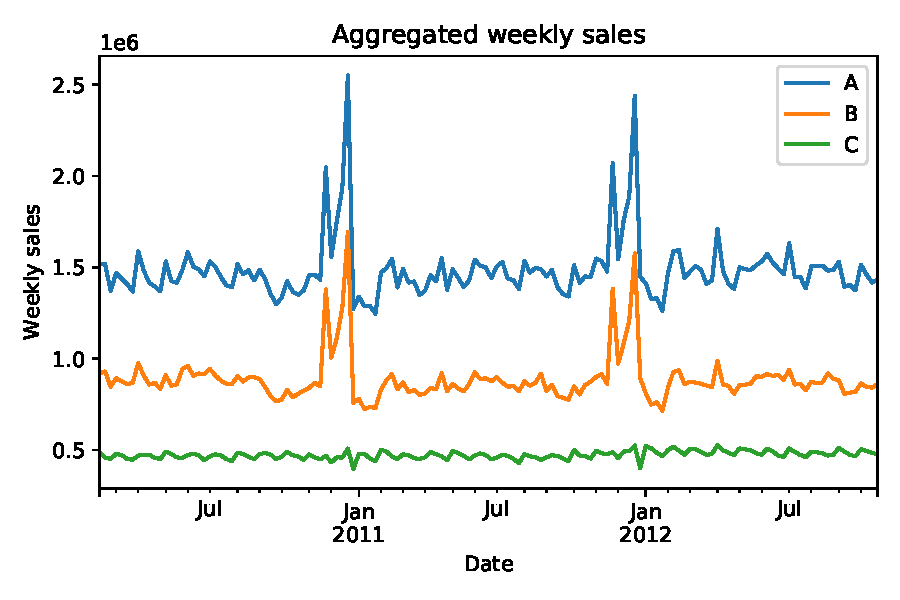
\includegraphics[height=8cm]{../plots/dataset/dataset_plot_y.pdf}
	\caption{Aggregated weekly sales by store group. Groups A and B demonstrate holiday effects while group C remains relatively stable through each year.
	}
	\label{fig:data_y}
\end{figure}

\begin{figure}[htb]
	\begin{subfigure}[b]{0.5\textwidth}
		\centering
		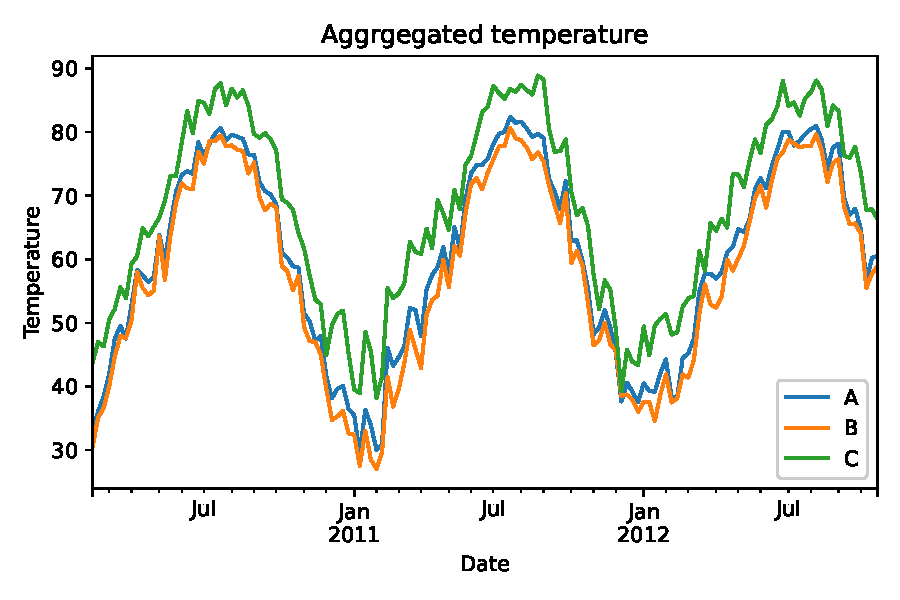
\includegraphics[width=\textwidth]{../plots/dataset/dataset_plot_temperature.pdf}
		\caption{Temperature by store group}
		\label{fig:data_temp}
	\end{subfigure}
	\hfill
	\begin{subfigure}[b]{0.5\textwidth}
		\centering
		\includegraphics[width=\textwidth]{../plots/dataset/dataset_plot_CPI.pdf}
		\caption{Consumer price index by store group}
		\label{fig:data_cpi}
	\end{subfigure}
	\begin{subfigure}[b]{0.5\textwidth}
		\centering
		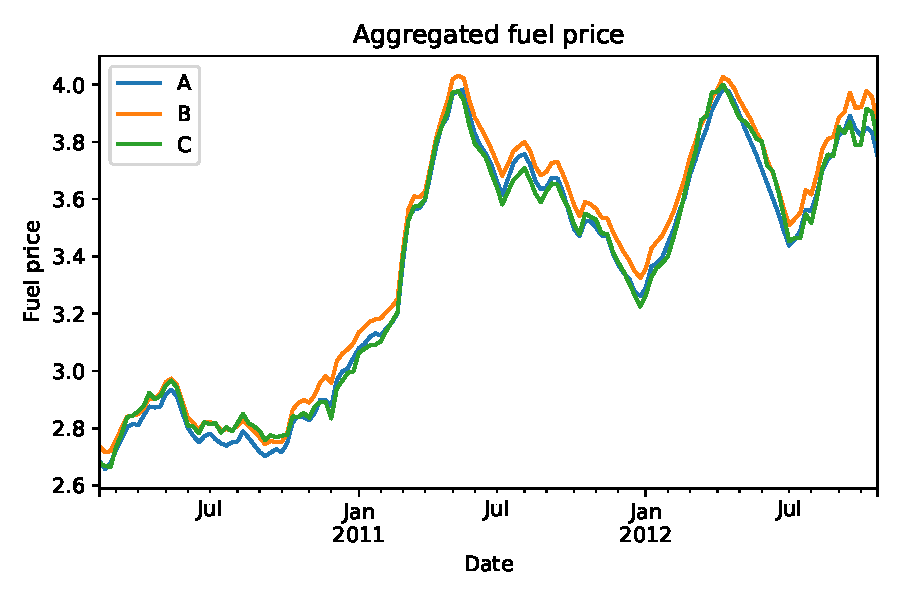
\includegraphics[width=\textwidth]{../plots/dataset/dataset_plot_fuel_price.pdf}
		\caption{Fuel price by store group}
		\label{fig:data_fuel}
	\end{subfigure}
	\hfill
	\begin{subfigure}[b]{0.5\textwidth}
		\centering
		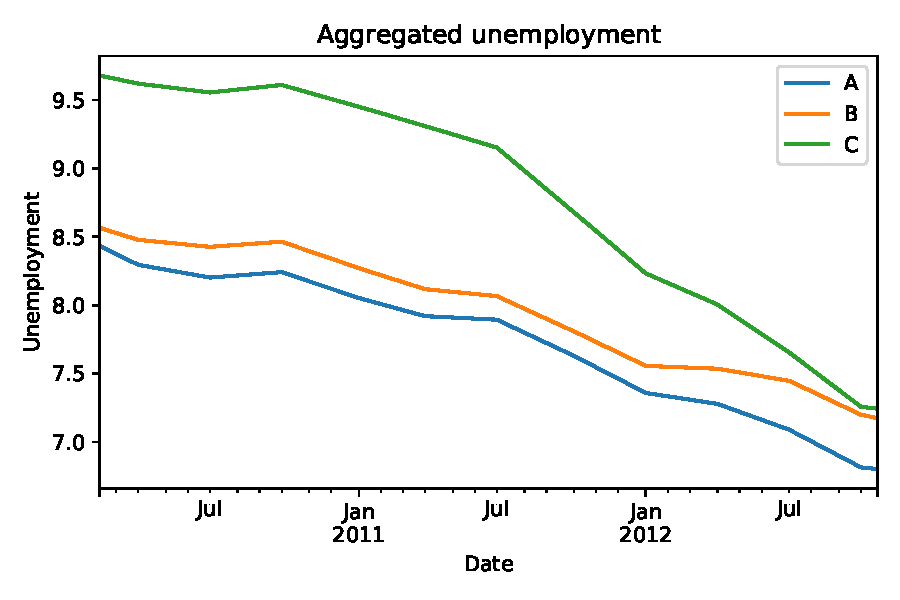
\includegraphics[width=\textwidth]{../plots/dataset/dataset_plot_unemployment_interpolated.pdf}
		\caption{Interpolated unemployment rate by store group}
		\label{fig:data_unemp}
	\end{subfigure}
	\caption{\label{fig:regressors} Additional features used in Model M2.}
\end{figure}

% Mallit

\subsection{Prophet-models}

The Prophet model by \cite{Prophet} is a linear model that is used to predict time series. The model consists of seasonality components, piece-wisely linear trend, and possible explanatory variables such as holidays. A component-wise breakdown of a fitted model is visualised in Fig. \ref{fig:prediction_components_demo}. The seasonalities are modelled using a Fourier approximation with a limited number of coefficients. Trend is modelled linearly between a number of pre-determined changepoints. After the last change point the model also assumes a linear trend. The prophet model treats time as a feature ranging from 0 to 1. Notably, the prediction does not directly depend on previous observations but seasonality and trend. They are calculated using also the other observations, but that calculation does not require a constant time difference between observations. As such, the model can handle inconsistent time intervals between datapoints. This means that the training and testing set do not have to consist of sequential observations.


Each of the five used models is an Prophet model with different settings and features. The models are labeled M1 to M5. The first model was chosen to act as a benchmark to be compared against the other models. This should demonstrate if changes to the base model yield any improved predictive performance. The second model adds on the benchmark model by also incorporating the additional features present in the dataset. These were temperature, CPI, unemployment rate and fuel price. The fourth model does not utilise the extra features. It attempts to demonstrate the behaviour of the metrics with overfitted models. The number of Fourier coefficients for seasonality are doubled from the benchmark model. Models three and five differ fundamentally from the other models as they are not reasonably possible to implement in a real world prediction scenario. Both of them are given the sales time series as an explanatory variable. This is done to study the behaviour of the metrics in situations where the models actually represent the real world data generating process. In this case the process is rather simple, as the correct prediction should follow trivially from the features. Model three is equal to the benchmark model extended by this feature. Model five has also less trend changepoints and disabled seasonality. As M5 should produce the exact same output with less variables the information criteria should always rank it as better performing. The differences between used models are displayed in Table \ref{tab:model_settings}.

% M1: Only weekly sales, no additional features.
% M2: All features, no other tricks.
% M3: The response variable is given as a explanatory variable. Perfect predictions can thus be obtained with this model.
% M4: Seasonality is modeled with 20 coefficients instead of 10.
% M5: Similar to M3, but seasonality is disabled, and trend has only one changepoint. 

\begin{table}[]
	\caption{\label{tab:model_settings} Different settings used in each model. Extra features are fuel price, CPI, unemployment and temperature.}
	\begin{tabular}{|l|l|l|l|l|l|}
		\hline
																		& \textbf{M1} & \textbf{M2} & \textbf{M3} & \textbf{M4} & \textbf{M5} \\ \hline
		Yearly seasonality coefficients & 10          & 10          & 10          & 20          & None        \\ \hline
		Extra features                  &             & X           &             &             &             \\ \hline
		Trend changepoints              & 25          & 25          & 25          & 25          & 1           \\ \hline
		Response variable as regressor  &             &             & X           &             & X           \\ \hline
		\end{tabular}
\end{table}


% Joku lörinä M-open, M-closed yms. jutuista olis aika hyvä just tässä.

% Metriikat

\subsection{Metrics}

The models were compared using five different metrics. The metrics used were Akaike information criterion (AIC), deviance information criterion (DIC), Watanabe-Aikaike information criterion (WAIC), mean average percentage error (MAPE), and 10-fold cross validation. The information criterions are calculated using only in-sample fits. They aim to estimate the out-of-sample predictive performance of the model using the likelihood of past observations. Notably only WAIC of the information criterions fully considers the bayesian nature of the model. It utilises the whole posterior distribution instead of some aggregated values. MAPE is calculated in the spirit of hold-out predictive methods by reserving a small portion of data from the tail of the dataset to act as a test set. The percentage errors of the predictions are then averaged to obtain MAPE. 10-fold cross validation is calculated by assigning randomly 1/10 of the datapoints as test set and then calculating the likelihood of the prediction for the test set. This is performed ten times so that each datapoint belongs to the test set once. 10-fold CV is the average of the results. Test set selection of MAPE is demonstrated in Fig. \ref{fig:hold_out_data} and one of the 10-fold cv splits can be found in Fig. \ref{fig:cv_demo}. 

\begin{figure}[htb]
	\centering
	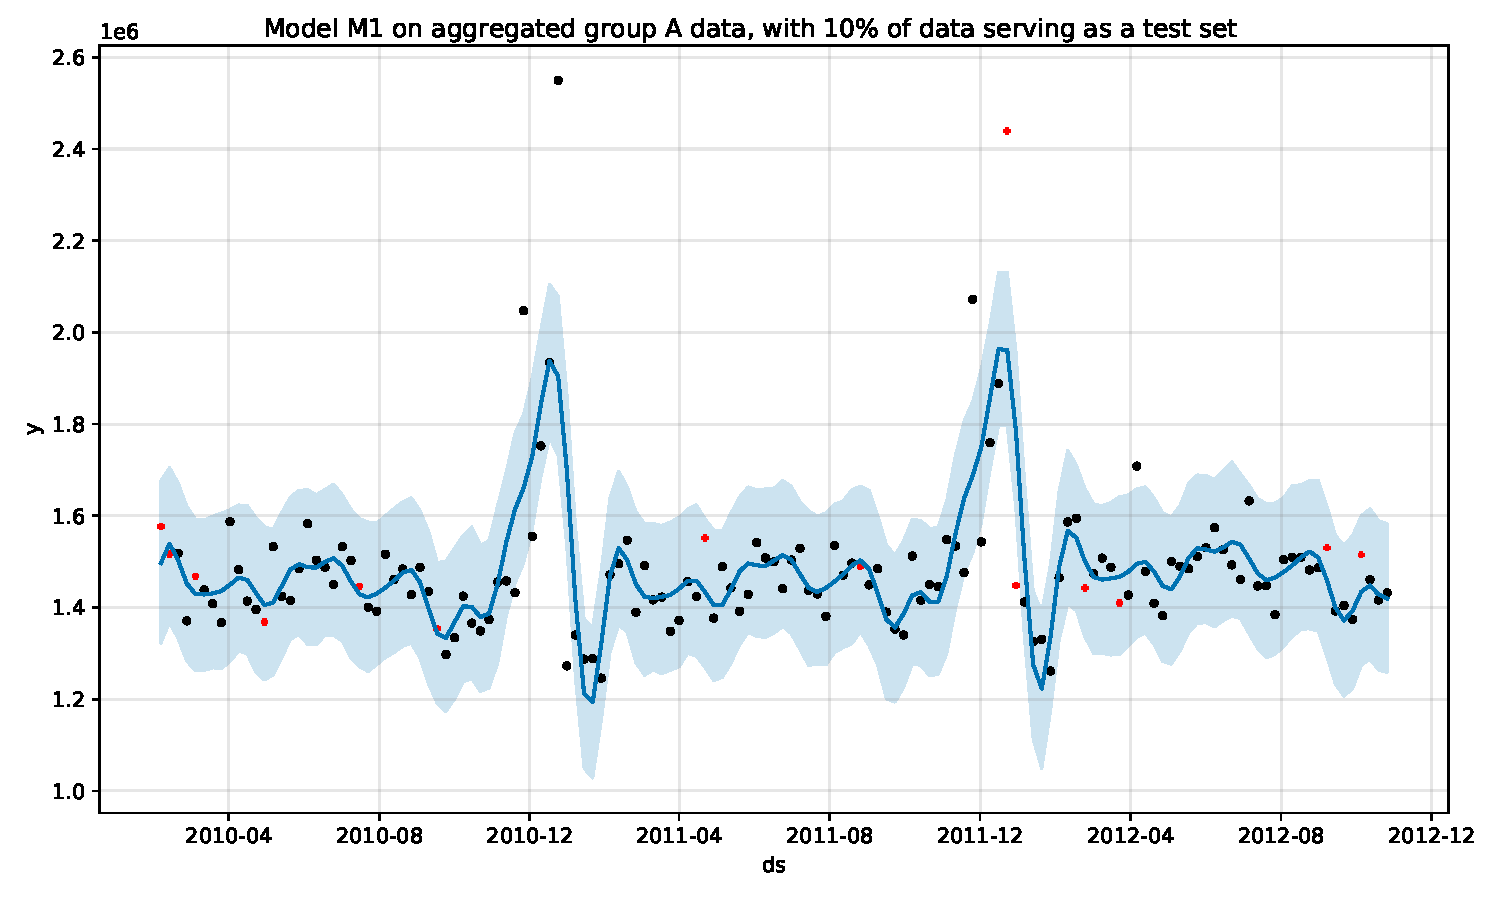
\includegraphics[height=8cm]{../plots/forecasts/cv_metric_demo_plot.pdf}
	\caption{Demonstrating the cv metric calculation. Red dots represent the 10\% of the datapoints that were selected for testing set. Model is fitted using training data represented
	by the black dots. This data splitting and evaluation is repeated ten times until all datapoints have belonged to the test set exactly once.}
	\label{fig:cv_demo}
\end{figure}

\begin{figure}[htb]
	\centering
	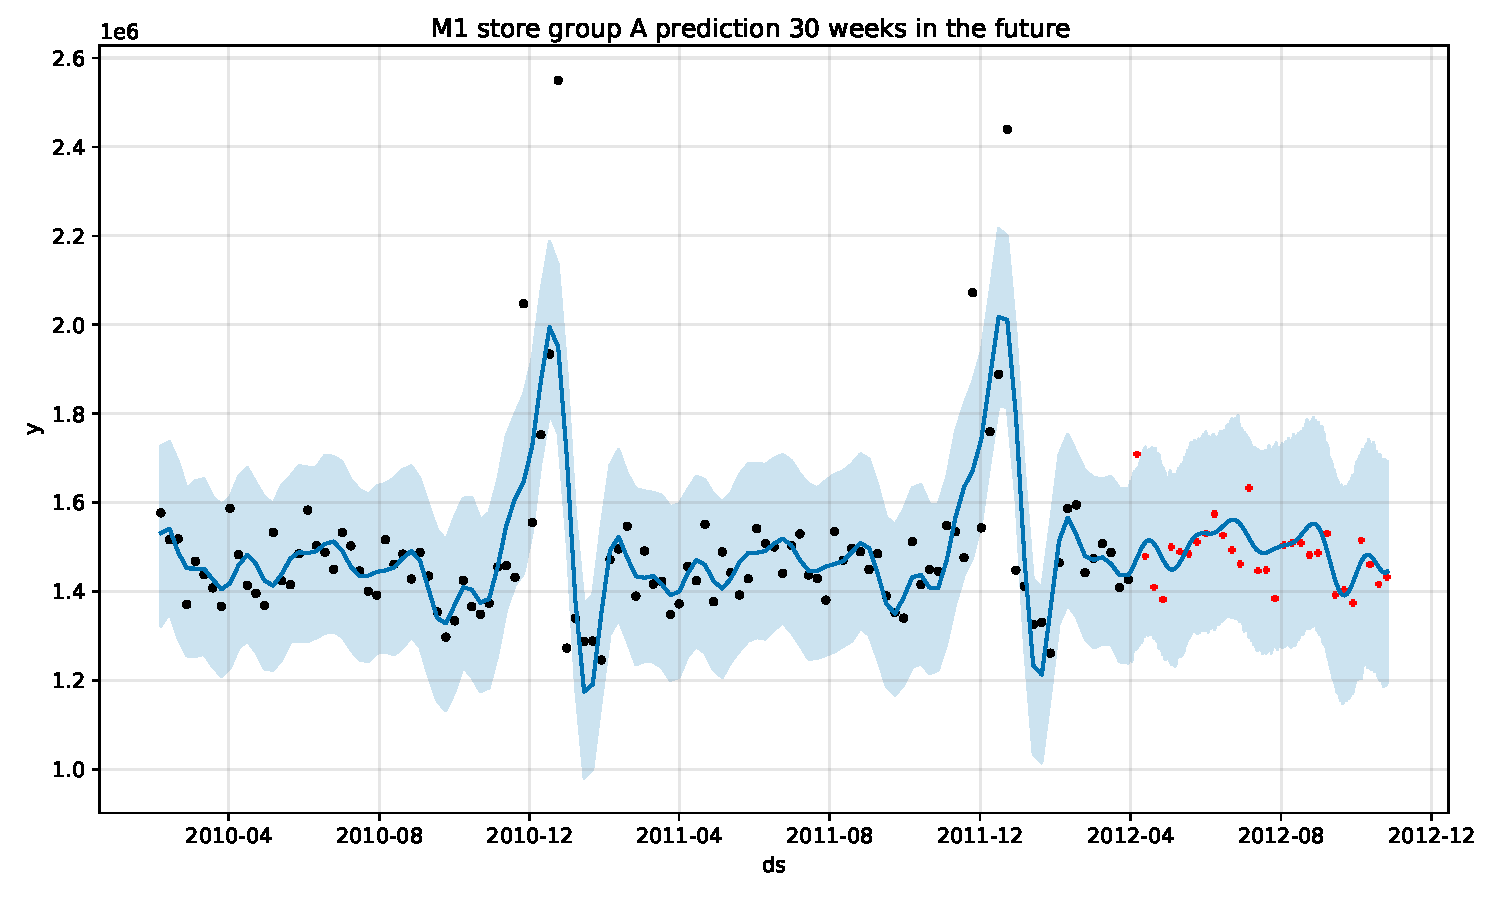
\includegraphics[height=8cm]{../plots/forecasts/30_weeks_prediction_demo.pdf}
	\caption{Hold-out prediction 30 weeks in the future. Training data in black, test data in red. This train / test split is used in MAPE metric.}
	\label{fig:hold_out_data}
\end{figure}

\begin{figure}[htb]
	\centering
	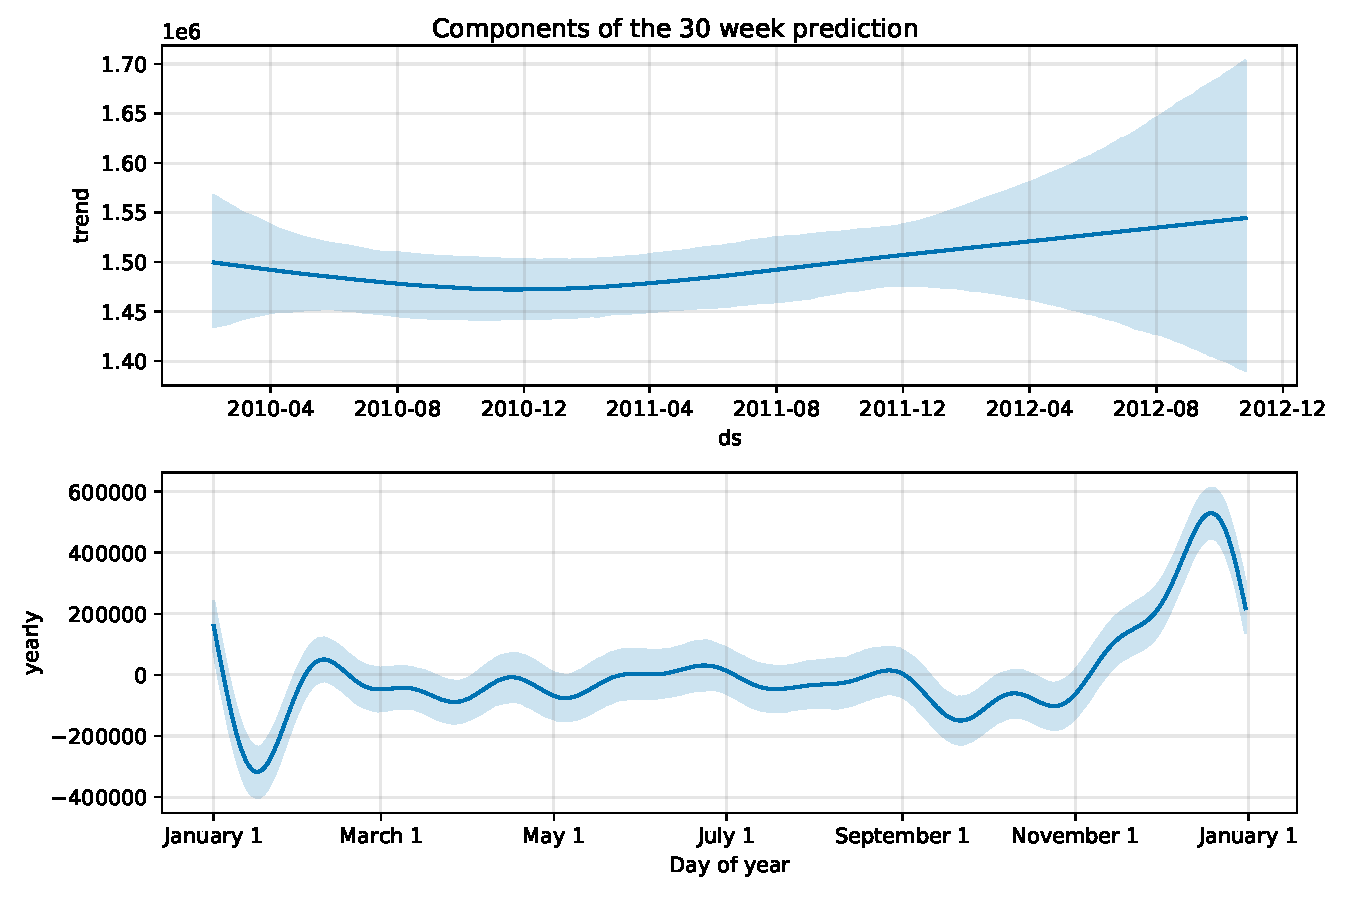
\includegraphics[height=8cm]{../plots/forecasts/30_weeks_prediction_components_demo.pdf}
	\caption{Trend and yearly seasonality components of the fitted model used in Fig. \ref{fig:hold_out_data}.}
	\label{fig:prediction_components_demo}
\end{figure}

\subsection{Bayesian model fitting}

Bayesian models rely on inferring the posterior probability densities of the parameters from data and prior probabilities. For complex models this can not be done analytically but by using Markov chain Monte Carlo sampling (MCMC). To be more specific, the adaptation of MCMC used in Stan was the No-U-Turn sampler (NUTS), as described in \cite{NUTS}. This sampling process explores the possible parameter space of the model, searching for likely parameter values, and yields a large collection of point value combinations for the parameters. Stan is a Bayesian data modelling platform used to mathematically model the Prophet model and fit it using MCMC sampling. Usually the sampling process utilises multiple chains to ensure proper convergence of the sampling process.

\subsection{Workflow}

This thesis focuses on the metrics used in model selection, not necessarily the model selection process itself. The workflow of metric evaluation was as follows: First the data was analysed to check for which features to use or if some data processing had to be done. After this the data was aggregated to different datasets: three by store group level and nine store level datasets. The compared models were constructed from the available data. Each of the models was fitted for each of the available datasets. Each of the five metrics were then computed for all the model-data combinations. All the fitted models and metrics were saved in a Pickle container to be analysed later. Ordering of the models by metrics results were then compared against each other within each dataset.

% Miten MAPE eroaa likelihood-jutuista

% Perustelut just näiden metriikoiden valinnalle

% Perustelu 10-fold cv:n datan droppaukselle, jossa ennustetta ei lasketa yhtenäiselle ajanjaksolle






% https://www.overleaf.com/learn/latex/How_to_Write_a_Thesis_in_LaTeX_(Part_3):_Figures,_Subfigures_and_Tables


% \begin{figure}[htb] % Kaikkien mallien in-sample -fitit
% 	\centering
% 	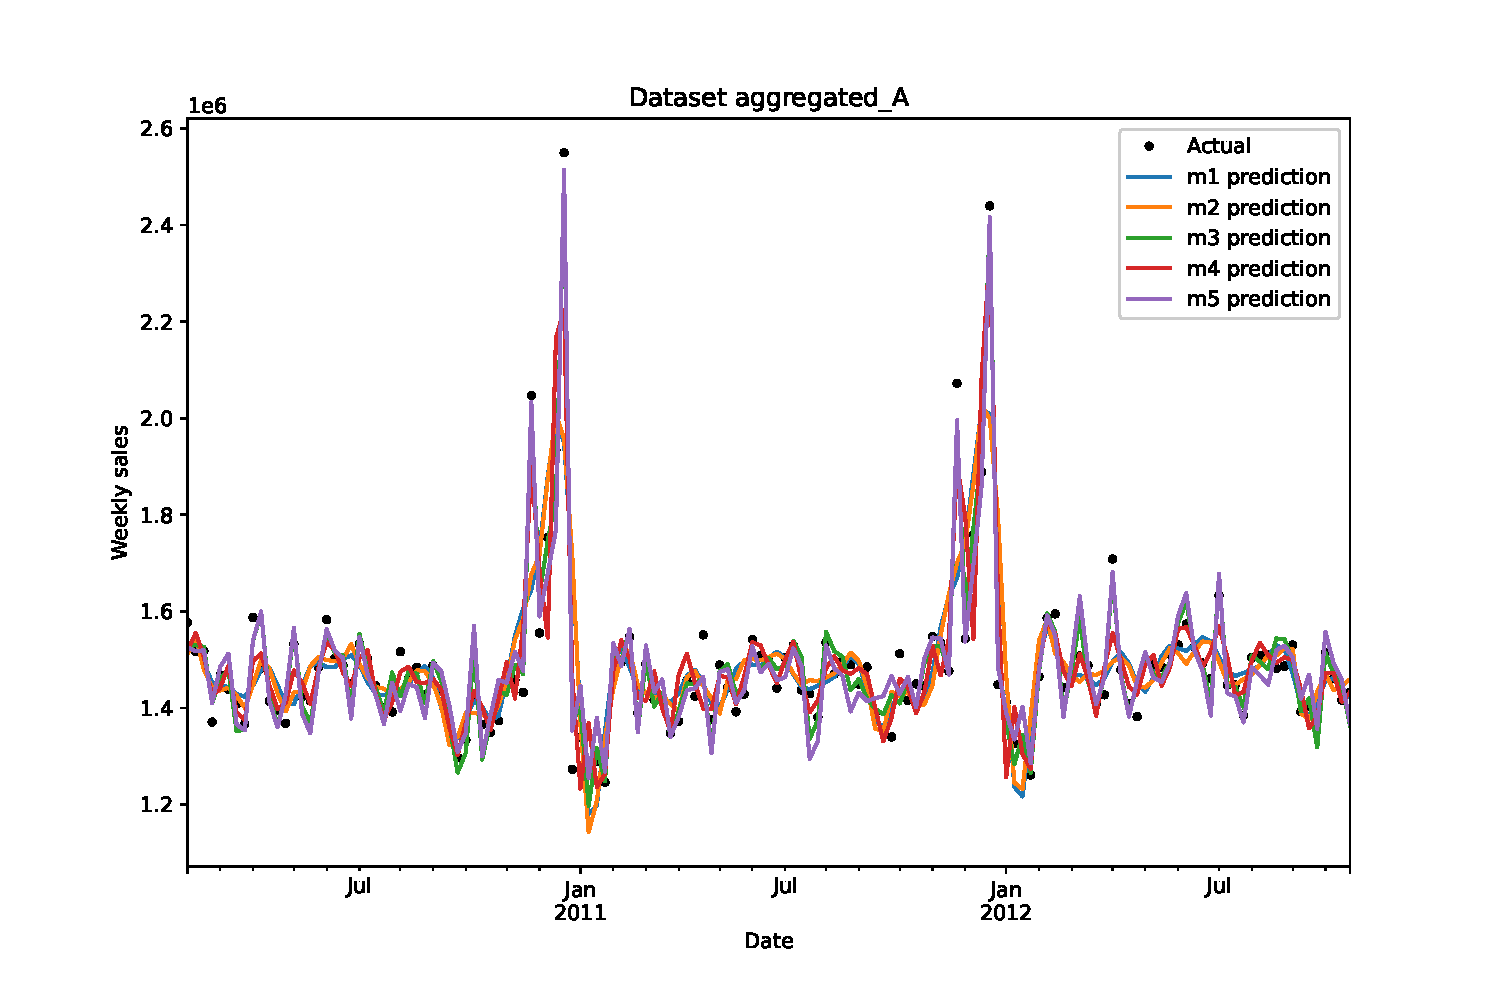
\includegraphics[height=8cm]{../plots/forecasts/model_fits_aggregated_A.pdf}
% 	\caption{A concept of what another kind of prediction plot could look like. This plot shows in-sample predictions from each of the models in one dataset.}
% 	\label{fig:plot_demo_2}
% \end{figure}


\section{Results}

% – Tuloksia voi havainnollistaa kuvilla ja taulukoilla 

% – Tulosten tulkinta esittelyn yhteydessä: Mitä tulokset tarkoittavat
% tutkittavan ilmiön kannalta? Ovatko ne järkeviä? Ovatko
% esimerkiksi tulokset tilastollisesti merkittäviä?

% – Herkkyystarkastelut – miten mallin oletukset / parametrivalinnat
% vaikuttavat tuloksiin?

% Tulosluvun tulee olla ymmärrettävissä ilman syvällistä
% perehtymistä menetelmälukuun – vältä yliteknisyyttä.

% Ensin laitetaan plotit ja taulukot omille paikoilleen



% Tässä osassa esitetään tulokset ja vastataan tutkielman alussa
% esitettyihin tutkimuskysymyksiin. Tieteellisen kirjoitelman
% arvo mitataan tässä osassa esitettyjen tulosten perusteella. 

%% Huomaa seuraavassa kappaleessa lainausmerkkien ulkopuolella piste, 
%% koska piste ei lopeta lainattua tekstinpätkää.
%% Jos lainattu tekstinpätkä loppuu välimerkkiin, tulee välimerkki
%% lainausmerkkien sisälle: 
%% "Et tu, Brute?" sanoi Caesar kuollessaan.
% Tutkimustuloksien merkitystä on aina syytä arvioida ja tarkastella
% kriittisesti.  Joskus tarkastelu voi olla tässä osassa, mutta se
% voidaan myös jättää viimeiseen osaan, jolloin viimeisen osan nimeksi
% tulee >>Tarkastelu>>. Tutkimustulosten merkitystä voi arvioida myös
% >>Johtopäätökset>>-otsikon alla viimeisessä osassa. 

% Tässä osassa on syytä myös arvioida tutkimustulosten luotettavuutta.
% Jos tutkimustulosten merkitystä arvioidaan >>Tarkastelu>>-osassa,
% voi luotettavuuden arviointi olla myös siellä. 


The models were fitted using Stan for MCMC sampling with four chains and sampling parameters target metropolis acceptance rate $\delta = 0.9$ and maximum tree depth of 11. Rest of the sampling parameters were left to their default values as suggested by Stan authors. The obtained results for the metrics are presented in Table \ref{tab:metrics_results}. Each of the used datasets produced a table of the same format, but only the tables for store-group level aggregation are presented here for clarity. More numerical results can be found in the Appendix. The columns of the tables represent the evaluated metrics. For the information criteria and MAPE evaluation lower values are desirable. As 10-fold CV is a likelihood, higher is better. The metric results can be used to rank the models by their performance. This is visualised in Fig. \ref{fig:metrics_visualization}. From the figure it can be seen that the results are somewhat consistent between the models and metrics.
% TODO: Lisää ne resultsit liitteeksi.

%\subsection{Metrics for the models}

The visual representation highlights the order different metrics rank the models. AIC and DIC ranked all the models similarly for all the datasets, but there were differences in the margins between the models. WAIC seemed to mostly agree with AIC and DIC, but in datasets B and C the order of models m1 and m4 was reversed. 

Ranking by MAPE has many similarities with the information criterion rankings. However the Model M5 performed worse with all datasets, dropping behind m3 in A and C, but also behind m1 and m4 in B. In dataset B MAPE ranked m1 better than m4. This agrees with the WAIC ranking, but it is the other way around with AIC and DIC. The other notable difference in MAPE scores is that in datasets A and B the Model M2 seems to perform much worse than the other models. However this phenomenon is not present in C. 

10-fold cross validation ranks the models m5 and m3 the best in all datasets, just like the information criterions do. However the ranking of the rest varies. In dataset C the models m1, m2 and m4 are ranked similarly as by AIC and DIC. In both A and B the Model M4 takes the last place, while m2 and m1 get a score similar to each other. M2 was ranked better than m1 for dataset A and vice versa for B, but the margin was rather slim.

% TODO: VOIKO OLLA NIIN, ETTÄ 10-FOLD CV:SSÄ KÄY M4:N KANSSA SITEN, ETTÄ VAAN JOKU NIISTÄ FITEISTÄ MENEE TOSI PAHASTI PIELEEN???

\subsection{Applicability of the metrics}


Overall it seems, that the metrics correctly recognise the "data generating models" from other models. Also M5 mostly ranks better than M3, as it has less non-informative regressors. When it comes to the ranking of models M1, M2 and M4, the results are not as clear. In store groups A and B M2 performs much worse than the other models when evaluating with MAPE. This likely indicates, that the model overestimates the importance of the external regressors. As the regressors have trends, the prediction drifts off the actual sales. In 10-fold cv this is not observed, as the datapoints in test set are picked randomly. The test points have similar-valued training points next to them, thus the trend does not have time to cause the predictions to drift off.

10-fold cv appears to rank M4 worse than the other metrics. This may be due to overfitting the seasonality with too little training data. As the model is evaluated with 10-fold cv, 10\% of the data is reserved for testing. This reduction of training data can be the cause for the model to overfit the seasonality, as it had a greater number of coefficients to fit than the other models.

% TODO: testaa molemmat yllä mainitut hypoteesit: MAPE:n ja cv:n erot, M4 overfittaus jos vaan 90% datasta käytössä

One thing to keep in mind when examining the results is the difference of loss functions used in the metrics, in particular the difference in MAPE and the others. Other metrics are based on estimating the log-likelihood of out-of-sample predictions, while MAPE evaluates the mean absolute percentage error. Log-likelihood is proportional to MSE as the model consist an normally distributed error term with a constant variance. In a perfect world the loss function would be representing the actual losses due to errors in predictions. However, it is really difficult to estimate those accurately. 


% Pohditaan syitä tuloksille 
% mitä tulokset tarkoittavat nyt sitten mallien validoinnin kannalta?
% - Onko järkevää käyttää *IC-metriikoita? Vai olisko MAPE sittenkin hyvä?
% - Muistutetaan lukijaa loss-functionin merkityksestä
% - lisätutkimus: loss-functioniks joku mapen tyyppinen, mut millä sit annetaan sakkoja?


\begin{table}
	\caption{\label{tab:metrics_results}Numerical representation of the validation metric results applied by store group.}
	\begin{subtable}[t]{\textwidth}
		\caption{\label{tab:metrics_A}Store group A}
		\csvreader[%
		tabular={|c|c|c|c|c|c|},
					table head = \hline\textbf{Model} &\textbf{AIC} &\textbf{DIC} &\textbf{WAIC} &\textbf{MAPE}&\textbf{10-fold CV}\\\hline,
					late after line= \\,
					late after last line=\\\hline %
					]{../tables/rounded/aggregated_A_metrics.csv}{model_name=\mname,DIC=\dic,AIC=\aic,WAIC=\waic,default_cv=\MAPE,10-fold_cv=\cv}%
					{\mname & \aic & \dic & \waic & \MAPE & \cv}
					\centering
					
	\end{subtable}

	\begin{subtable}[t]{\textwidth}
		\caption{\label{tab:metrics_B}Store group B}
		\csvreader[%
		tabular={|c|c|c|c|c|c|},
					table head = \hline\textbf{Model} &\textbf{AIC} &\textbf{DIC} &\textbf{WAIC} &\textbf{MAPE}&\textbf{10-fold CV}\\\hline,
					late after line= \\,
					late after last line=\\\hline %
					]{../tables/rounded/aggregated_B_metrics.csv}{model_name=\mname,DIC=\dic,AIC=\aic,WAIC=\waic,default_cv=\MAPE,10-fold_cv=\cv}%
					{\mname & \aic & \dic & \waic & \MAPE & \cv}
					\centering
					
	\end{subtable}

	\begin{subtable}[t]{\textwidth}
		\caption{\label{tab:metrics_C}Store group C}
		\csvreader[%
		tabular={|c|c|c|c|c|c|},
					table head = \hline\textbf{Model} &\textbf{AIC} &\textbf{DIC} &\textbf{WAIC} &\textbf{MAPE}&\textbf{10-fold CV}\\\hline,
					late after line= \\,
					late after last line=\\\hline %
					]{../tables/rounded/aggregated_C_metrics.csv}{model_name=\mname,DIC=\dic,AIC=\aic,WAIC=\waic,default_cv=\MAPE,10-fold_cv=\cv}%
					{\mname & \aic & \dic & \waic & \MAPE & \cv}
					\centering
	\end{subtable}
\end{table}

\begin{figure}
	\begin{subfigure}[htb]{0.5\textwidth}
		\centering
		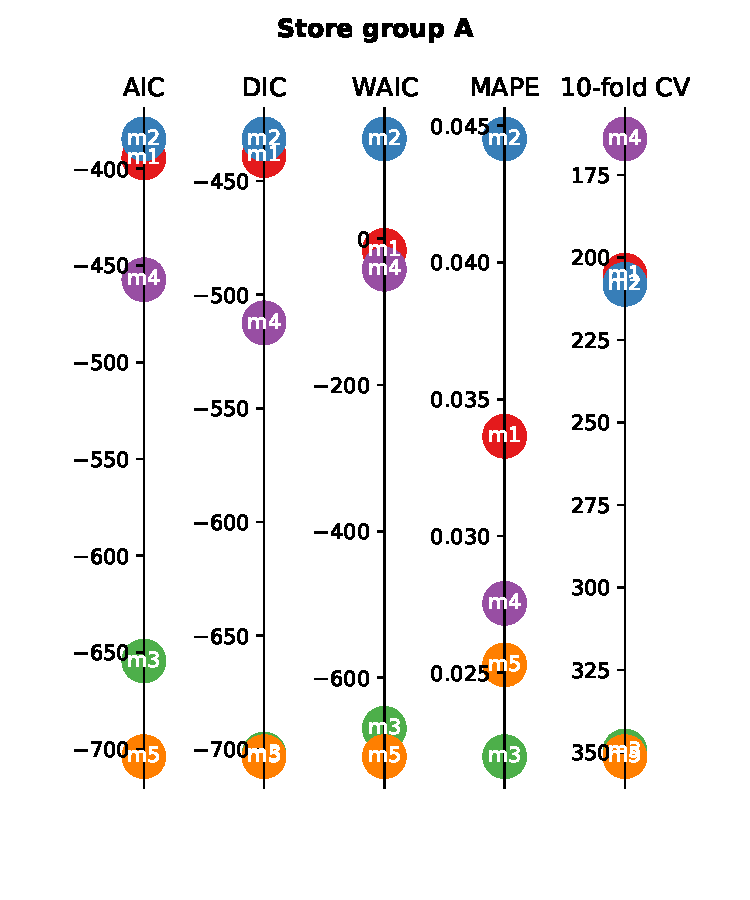
\includegraphics[width=\textwidth]{../plots/metrics/metrics_plot_A.pdf}
		\caption{Store group A}
		\label{fig:metrics_A}
	\end{subfigure}
	\hfill
	\begin{subfigure}[htb]{0.5\textwidth}
		\centering
		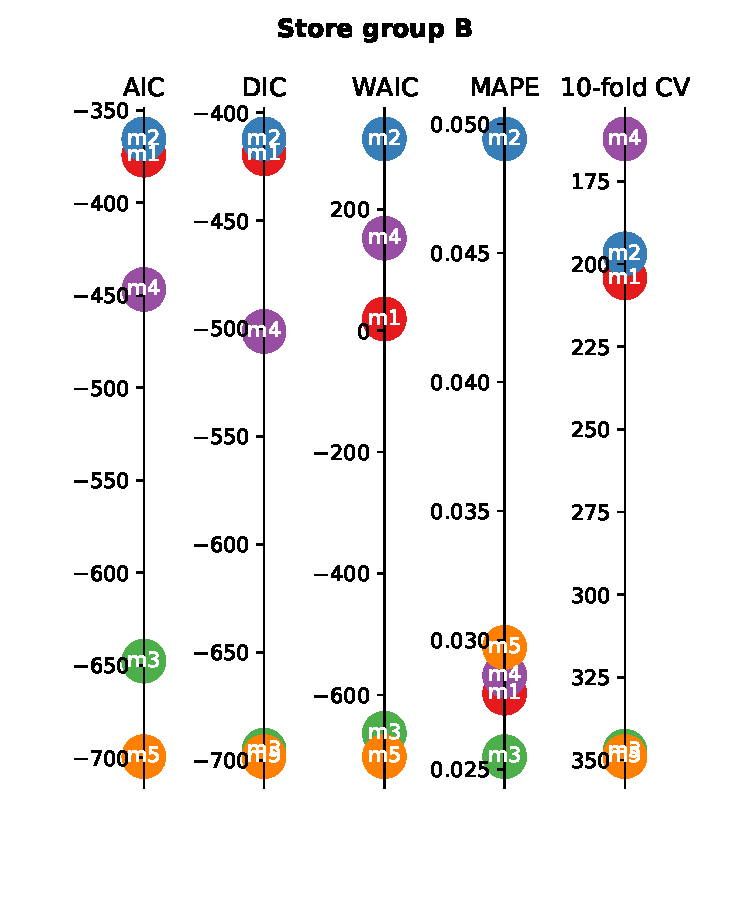
\includegraphics[width=\textwidth]{../plots/metrics/metrics_plot_B.pdf}
		\caption{Store group B}
		\label{fig:metrics_B}
	\end{subfigure}
	
	\begin{subfigure}[htb]{0.5\textwidth}
		\centering
		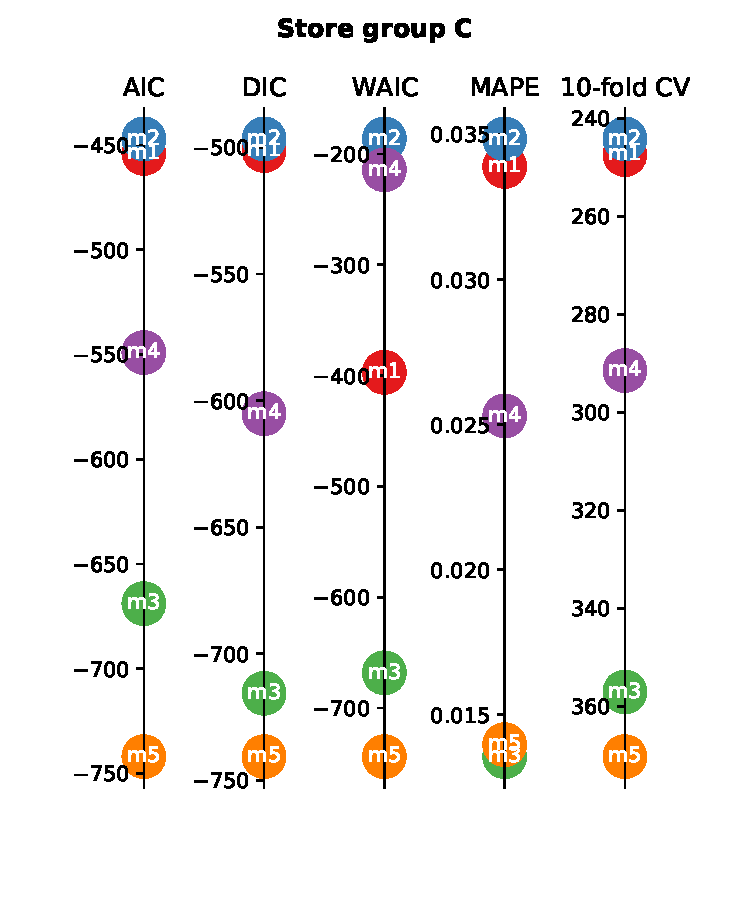
\includegraphics[width=\textwidth]{../plots/metrics/metrics_plot_C.pdf}
		\caption{Store group C}
		\label{fig:metrics_C}
	\end{subfigure}
	\caption{\label{fig:metrics_visualization}Visualisation of model validation metric results by store group. Arranged such that visually lower is better.
	Each axis is scaled so that extreme values are at the ends. Please note the inverted axis of 10-fold cross validation metric. For 
	precise values please refer to Table \ref{tab:metrics_results}}
\end{figure}






\section{Summary} 




% Ladataan library.bib
\clearpage
\bibliography{library}


%% Liitteet
%% Poista a.o. \clearpage- ja \thesisappendix -makrot, jos liiteitä ei ole.

\clearpage
\thesisappendix

\section{Numerical results for single stores\label{app:single_store_results}}

\begin{figure}
	\begin{subfigure}[htb]{0.33\textwidth}
		\centering
		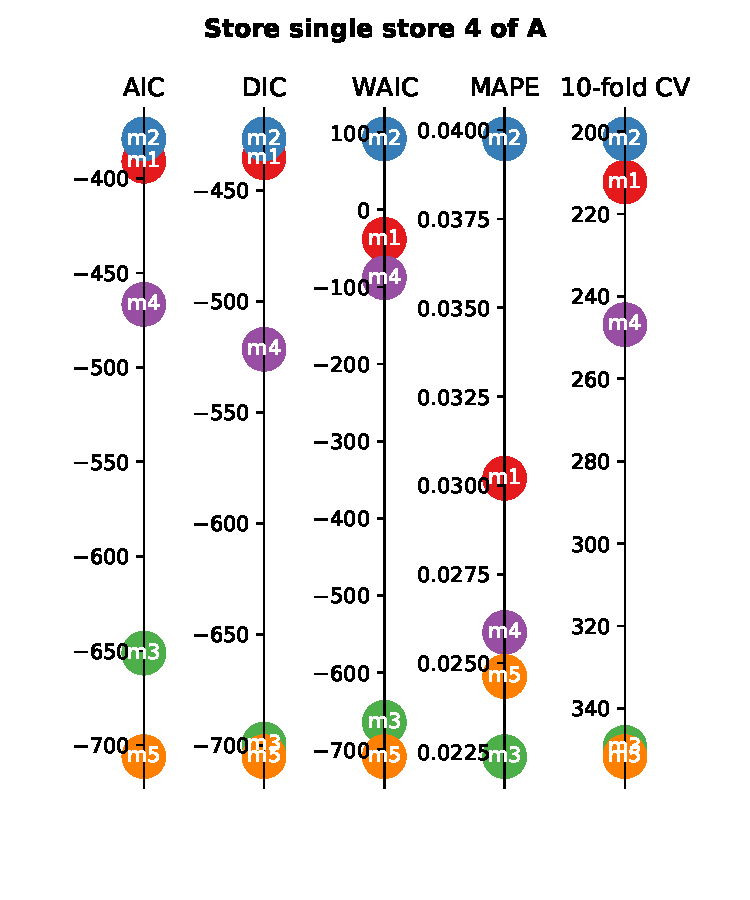
\includegraphics[width=\textwidth]{../plots/metrics/metrics_plot_single_store_4_of_A.pdf}
		%\caption{Store group A}
		%\label{fig:metrics_A}
	\end{subfigure}
	%\hfill
	\begin{subfigure}[htb]{0.33\textwidth}
		\centering
		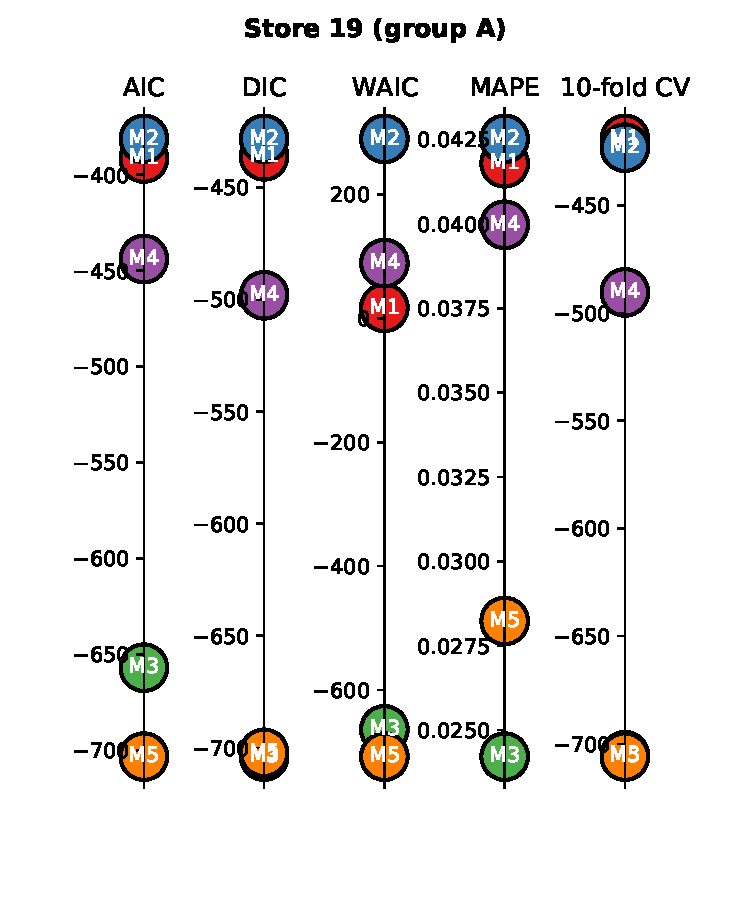
\includegraphics[width=\textwidth]{../plots/metrics/metrics_plot_single_store_19_of_A.pdf}
		%\caption{Store group B}
		%\label{fig:metrics_B}
	\end{subfigure}
	%\hfill
	\begin{subfigure}[htb]{0.33\textwidth}
		\centering
		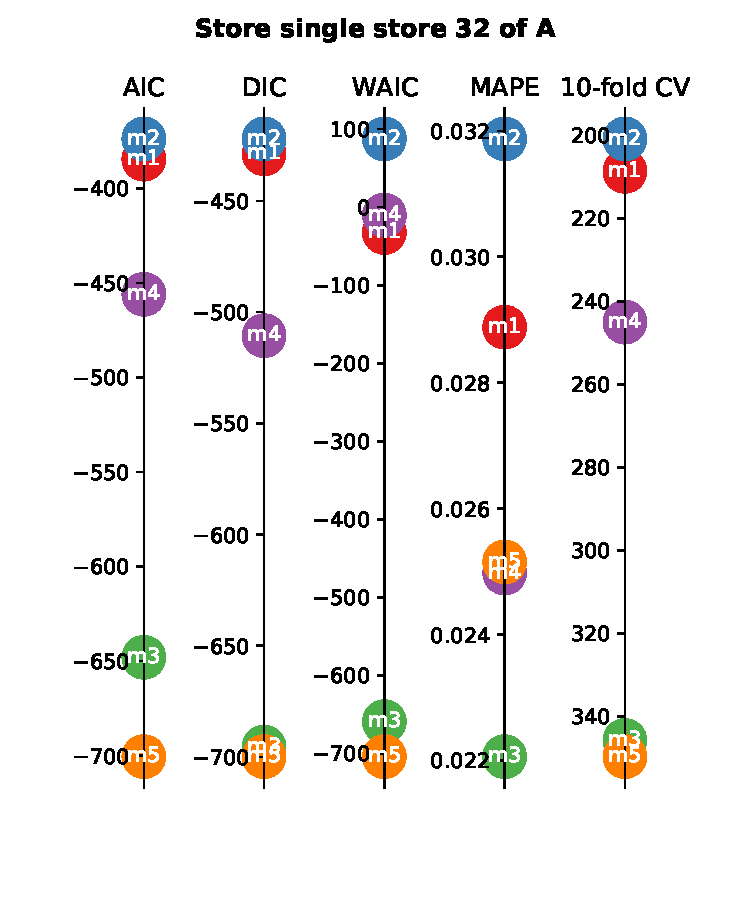
\includegraphics[width=\textwidth]{../plots/metrics/metrics_plot_single_store_32_of_A.pdf}
		%\caption{Store group B}
		%\label{fig:metrics_B}
	\end{subfigure}
	
	\begin{subfigure}[htb]{0.33\textwidth}
		\centering
		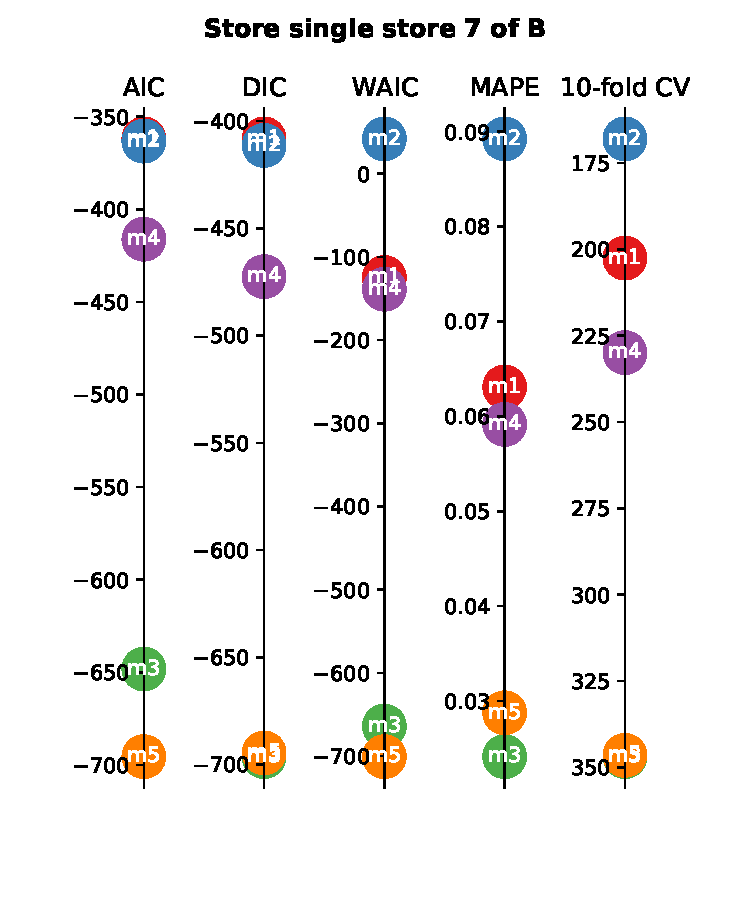
\includegraphics[width=\textwidth]{../plots/metrics/metrics_plot_single_store_7_of_B.pdf}
		%\caption{Store group A}
		%\label{fig:metrics_A}
	\end{subfigure}
	%\hfill
	\begin{subfigure}[htb]{0.33\textwidth}
		\centering
		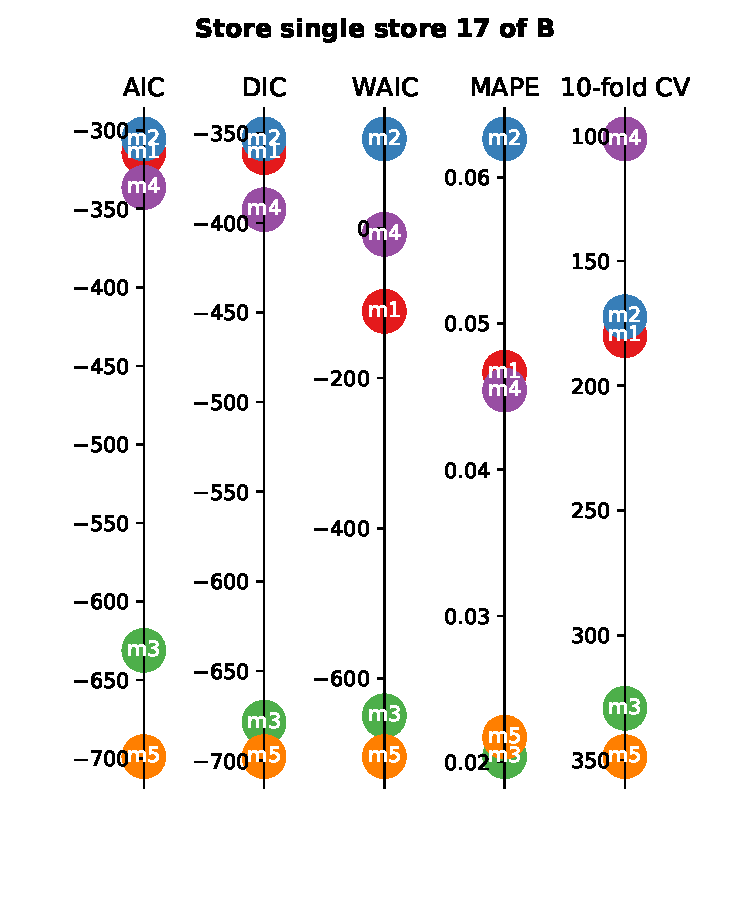
\includegraphics[width=\textwidth]{../plots/metrics/metrics_plot_single_store_17_of_B.pdf}
		%\caption{Store group B}
		%\label{fig:metrics_B}
	\end{subfigure}
	%\hfill
	\begin{subfigure}[htb]{0.33\textwidth}
		\centering
		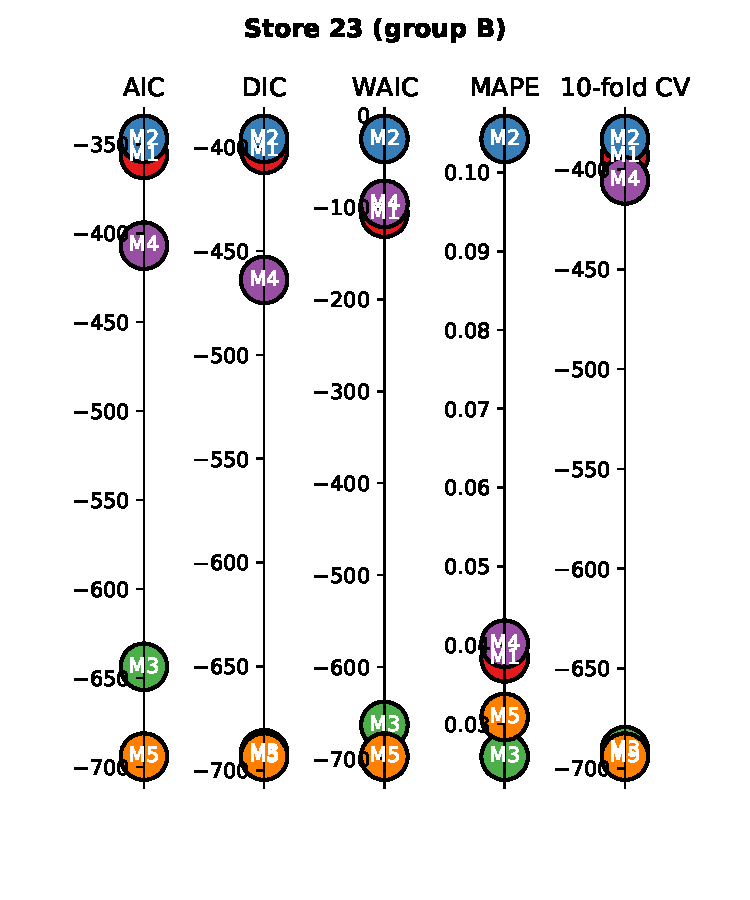
\includegraphics[width=\textwidth]{../plots/metrics/metrics_plot_single_store_23_of_B.pdf}
		%\caption{Store group B}
		%\label{fig:metrics_B}
	\end{subfigure}

	\begin{subfigure}[htb]{0.33\textwidth}
		\centering
		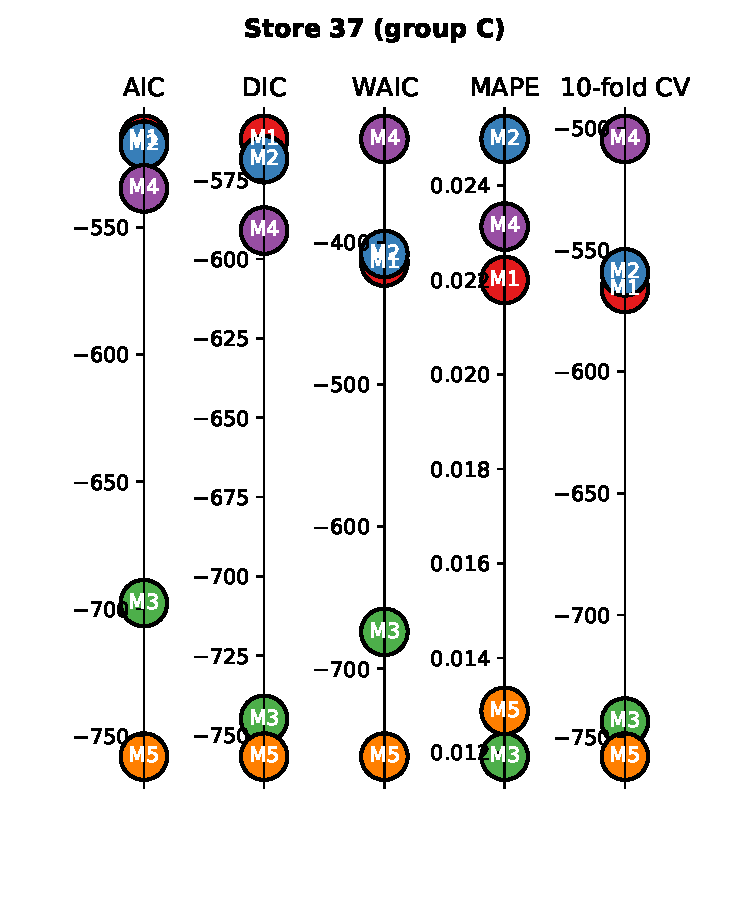
\includegraphics[width=\textwidth]{../plots/metrics/metrics_plot_single_store_37_of_C.pdf}
		%\caption{Store group A}
		%\label{fig:metrics_A}
	\end{subfigure}
	\hfill
	\begin{subfigure}[htb]{0.33\textwidth}
		\centering
		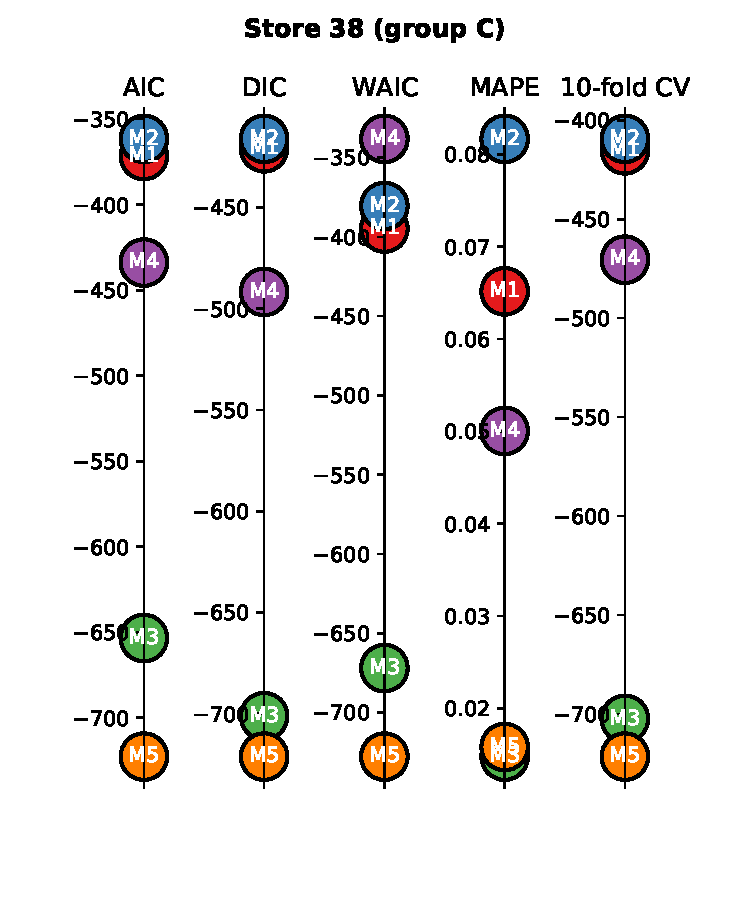
\includegraphics[width=\textwidth]{../plots/metrics/metrics_plot_single_store_38_of_C.pdf}
		%\caption{Store group B}
		%\label{fig:metrics_B}
	\end{subfigure}
	\hfill
	\begin{subfigure}[htb]{0.33\textwidth}
		\centering
		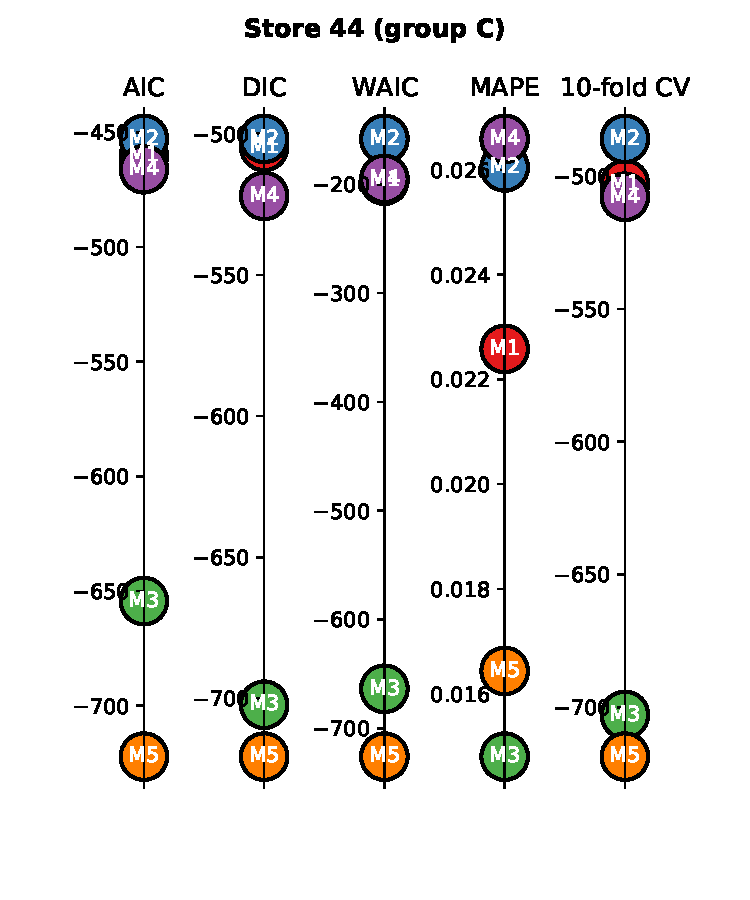
\includegraphics[width=\textwidth]{../plots/metrics/metrics_plot_single_store_44_of_C.pdf}
		%\caption{Store group B}
		%\label{fig:metrics_B}
	\end{subfigure}
	\caption{\label{fig:single_store_results_visualisation}Visualisation of model validation metric results for single stores.}
\end{figure}

%Kaavojen numerointi muodostaa liitteissä oman kokonaisuutensa:
%\begin{align}
%d \wedge A &= F, \label{liitekaava1}\\
%d \wedge F &= 0. \label{liitekaava2}
%\end{align}


%\clearpage
%\section{Toinen esimerkki liitteestä\label{LiiteB}}

%% Liitteiden kaavat, taulukot ja kuvat numeroidaan omana kokonaisuutenaan

% Liitteissä voi myös olla kuvia, jotka
% eivät sovi leipätekstin joukkoon:
%% Ympäristön figure parametrit htb pakottavat
%% kuvan tähän, eikä LaTeX yritä siirrellä niitä
%% hyväksi katsomaansa paikkaan. 
%% Ympäristöä center voi käyttää \centering-
%% komennon sijaan
%%

%%
% Liitteiden taulukoiden numerointi on kuvien ja kaavojen kaltainen:
% \begin{table}[htb]
% \caption{Taulukon kuvateksti.}
% \label{liitetaulukko}
% \centering
% \fbox{
% \begin{tabular}{lp{0.5\linewidth}}
% 9.00--9.55  & Käytettävyystestauksen tiedotustilaisuus (osanottajat
% ovat saaneet sähköpostitse valmistautumistehtävät, joten tiedotustilaisuus
% voidaan pitää lyhyenä).\\
% 9.55--10.00 & Testausalueelle siirtyminen
% \end{tabular}}
% \end{table}
% Kaavojen numerointi muodostaa liitteissä oman kokonaisuutensa:
% \begin{align}
% T_{ik} &= -p g_{ik} + w u_i u_k + \tau_{ik},  \label{liitekaava3} \\
% n_i    &= n u_i + v_i.                      \label{liitekaava4}
% \end{align}

\end{document} 
